This is a report for \jira{DM-22806} on automating the process to take LSST science pipelines outputs, produce parquet files, conform to the Science Data Model (SDM) format, and ingest them into Qserv.
The Qserv instance is deployed at NCSA accessible directly for LSST developers and via Science Platform for users.

The User Guide of the Qserv Ingest System is at \url{https://confluence.lsstcorp.org/x/WoPyBw}, where one can find detailed documentations on the Qserv Ingest APIs, example usages of the Ingest System, example workflows, and advanced ingest scenarios.
This DMTN does not intend to duplicate the User Guide; instead, this DMTN focuses on the end-to-end workflow starting with LSST science pipelines outputs and the current prototype system as implemented specifically for the NCSA environments.

\section{Input data from Science Pipelines}
The input data are the reprocessed HSC products available at Rubin's GPFS space \texttt{/datasets/hsc/repo/rerun/}.
The object tables produced by the postprocessing pipeline, part of the DRP processing, are used.
These object tables, with the Butler dataset type of \texttt{objectTable\_tract}, are provided one file per tract in the parquet format on the shared filesystem.
In the case of the HSC-RC2 dataset, there are three tracts in total, hence three parquet files are provided in each reprocessing rerun.


\section{Overall workflow}
Figure \ref{fig:workflow} illustrates the overall workflow from the input parquet files to an ingested database in the Qserv instance.

\begin{figure}[h]
  \centering
  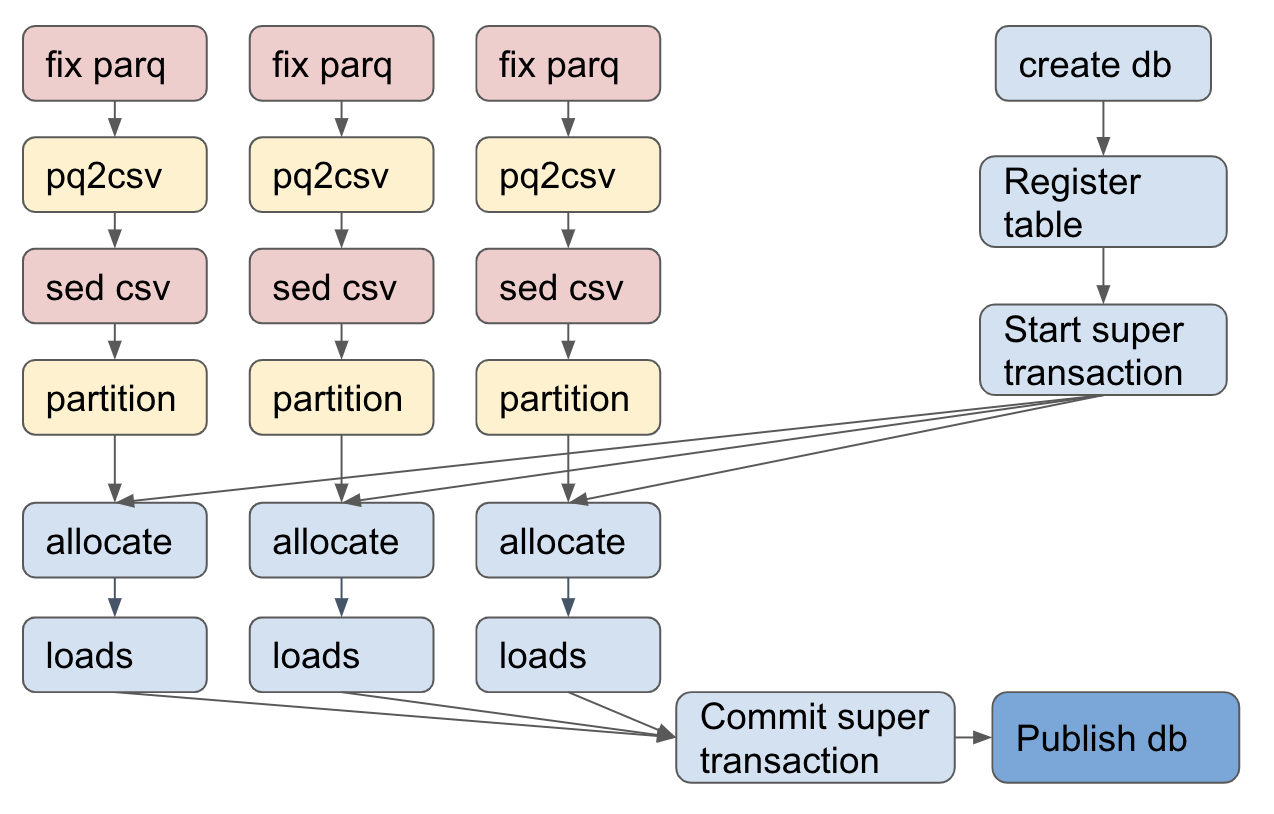
\includegraphics[width=0.70\textwidth]{ingest_workflow_DM27383.png}
  \caption{Workflow Diagram. Blue boxes indicate direct connections with the Qserv cluster; red boxes indicate temporary workarounds.}
  \label{fig:workflow}
\end{figure}

Constrained by the workflow management systems provided to DM developers on the Rubin Batch Systems \footnote{\url{https://developer.lsst.io/services/batch.html}}, the ingest workflow is implemented with Pegasus \footnote{\url{http://pegasus.isi.edu/}} for running on the HTCondor DAC Cluster.
The workflow code is at \url{https://github.com/lsst-dm/qserv-ingest-hsc-poc}.
The following sessions dive into individual steps of the workflow.


\section{Conforming parquet files to SDM}
The schema definitions of the Rubin Science Data Model (SDM) are felis-\footnote{\url{https://github.com/lsst-dm/felis}}-style YAML files and stored in the \texttt{sdm\_schemas} package \footnote{\url{https://github.com/lsst/sdm\_schemas}}.
The package is versioned with the \texttt{lsst\_distrib} stack.
In \texttt{ci\_hsc\_gen2}, the column names of the pipeline outputs are verified against the \texttt{sdm\_schemas/yml/hsc.yml} file.
As of this writing, the data types in the parquet files do not perfectly match SDM yet.
One issue is null handling.
While the convention to handle missing data is being discussed (\jira{DM-25926}) and the parquet files do not have SDM types, a step is added in the workflow to replace all nulls with 0 and to set column types following \texttt{sdm\_schemas/yml/hsc.yml}.


\section{Converting parquet to csv}
The \texttt{parquet\_tools} package \footnote{\url{https://github.com/lsst-dm/parquet\_tools}} is used to convert parquet files into csv format.
\texttt{pq2csv} expects a schema file and also checks the schema consistency with the input parquet files.
Currently \texttt{pq2csv} expect this schema in its own customized format, not felis.


\section{Fixing csv}
Boolean values should be represented by literals, so \texttt{Ture} and \texttt{False} are replaced by \texttt{1} and \texttt{0}.
Currently, \texttt{inf} and \texttt{-inf} are replaced by null values (\texttt{\textbackslash N}).
The linux \texttt{sed} command is used.


\section{Partitioning into chunk files}
The spatial data partition is performed by the \texttt{partition}\footnote{\url{https://github.com/lsst/partition}} package.
Output chunk files are directly stored onto the GPFS shared filesystem and are not tracked by the workflow manager.


\section{Using Qserv Ingest web services}
Qserv Ingest web services have REST APIs and the HTTP requests may be sent directly or via python code.
Our ingest client code is written in python utilizing the \texttt{requests} library.
Most requests expect a JSON object for the parameters.
These requests allow users to create a database, create a table, start a super-transaction, allocate chunks, commit a super-transaction, publish a database, and so on.
Suitable ports have been opened between the Rubin Batch Systems and the Qserv cluster to allow these HTTP requests.


\label{sec:loading}
\section{Data loading}
There are two ways to load data.
Previously, the binary tool \texttt{qserv-replica-file-ingest} available via the docker container was used. Due to the need of docker, it cannot be run on the clusters of the Rubin Batch Systems. Therefore, we did this step on Qserv machines on either masters or workers.
Recently, a new feature has been added (\jira{DM-27091}) for the workers to ingest files directly from the mounted filesystem, or by pulling from a remote object store. The Qserv workers now have built-in REST servers to load the data.  The new feature allows data loading to be done from the Rubin Batch Systems where docker cannot be used.

No data movement of the chunk files is involved as the chunk files are stored on the GPFS shared filesystem mounted on both the Rubin Batch Systems and the Qserv cluster.

\section{Examples}
Table \ref{tab:examples} lists the databases availabe in the "small" Qserv instance at NCSA as of this writing.
New object tables from the periodic HSC-RC2 reprocessing continue to be ingested into Qserv.
Some of these databases were ingested before the new data loading feature was implemented and the data loading was done on the Qserv cluster (see Sect \ref{sec:loading}), hence the job counts differ among the HSC-RC2 databases.
\texttt{w\_2020\_42} was the first HSC-RC2 database with data loading directly issued on the Rubin Batch Systems.
Some, but not all, of these databases are made queryable via TAP on Rubin Science Platform hosted at NCSA.

\begin{table}
\tiny
\centering
\begin{tabular} {|r|r|r|r|r|r|r|r|}
\hline
{Database Name}&{Dataset}&{Row Count}&{Input Size}&{Tract Count}&{Job Count}&{Wall time}&{Cumulative time}
\\ \hline
{hsc\_pdr2\_2020\_08\_01} & HSC-PDR2 DEEP & 32193313  & 45G & 39  & 198 & $\sim$32m & $\sim$5h39m \\
{hsc\_pdr2\_2020\_09\_00} & HSC-PDR2 WIDE & 570287192 & 659G & 663 & 3318 & 6h27m & 5d9h \\

{hsc\_rc2\_w\_2020\_30\_04} & HSC-RC2 & 5520644 & 8G & 3 & 18 & 26m & 1h1m  \\
{hsc\_rc2\_w\_2020\_38\_04} & HSC-RC2 & 5528373 & 8G & 3 & 18 & 25m & 1h3m \\
{hsc\_rc2\_w\_2020\_42\_05} & HSC-RC2 & 5516628 & 8G & 3 & 21 & 29m & 1h13m \\

{hsc\_rc2\_v21\_0\_0\_rc1\_04 } & HSC-RC2 & 5525413 & 8G & 3 & 21 & 29m & 1h13m \\
{hsc\_rc2\_w\_2021\_02\_00} & HSC-RC2 & 5516315 & 8G & 3 & 21 & 27m & 1h9m \\

{dc2\_object\_run22i\_dr6\_wfd\_v1\_08} & DC2 DR6 WFD & 147088445 & 118G & 166 & 999 & 47m & 11h23m \\
\hline
\end{tabular}
\caption{
An overview of current databases available in the "small" Qserv instance at NCSA.
These databases contain Object tables.
The job count, wall time, and cumulative job wall time of the ingest workflow for each batabase are also shown.
The workflow job counts do not include additional data transfer or management jobs added by the workflow manager Pegasus.
The timing information is provided by Pegasus.
The $\sim$ symbol indicates missing timing data; estimates are given.
The input size is the sum of all input parquet files.
One DC2 database is included for comparison.
}
\label{tab:examples}
\end{table}

